\section{Putting everything together}\label{sec:hierarchy}
 
%In this section we will combine \cref{thm:crossed-one-side} and \cref{thm:cutsbothsideswithinside} with one of the main results from ~\cite{KKO21} to prove \cref{thm:main}. We note that this section, similar to the proof of \cref{thm:crossed-one-side}, is not conceptually different from ~\cite{KKO21}.

In this section we use the following theorem to demonstrate \cref{thm:main}. While the proof of \cref{thm:maintechnical} is non-trivial, using \cref{thm:cutsbothsideswithinside} it follows from statements in \cite{KKO21} and does not require any new ideas. For this reason, we sketch the proof in this section, leaving the formal proof to \cref{app:proofbeforetechnical}. 

It turns out not to be useful to prove \cref{thm:hierarchyKKO} directly, but is an immediate corollary of the following theorem (we stated \cref{thm:hierarchyKKO} in the overview to improve readability and highlight the importance of \cref{thm:cutsbothsideswithinside}).

%One can see this theorem as a combination of \cref{thm:cutsbothsideswithinside} and \cref{thm:hierarchyKKO}, where the latter is a combination (and slight modification) of two theorems in \cite{KKO21}. Note we do not formally prove \cref{thm:hierarchyKKO} in this paper in order to more closely follow the proof template of \cite{KKO21}; it is instead used to help give intuition in the \cref{sec:overview}. However it can be proved in a nearly identical manner to the below by simply ``leaving out" the slack vector constructed in \cref{thm:cutsbothsideswithinside}. 

%The main goal of the section will be to show the following theorem. We set . 

\begin{restatable}[Combination of \cref{thm:hierarchyKKO} and \cref{thm:cutsbothsideswithinside}]{theorem}{maintechnical}\label{thm:maintechnical}
Let $x^0$ be a solution of LP \eqref{eq:tsplp} with support $E_0=E\cup \{e_0\}$, and $x$ be $x^0$ restricted to $E$.
Let $\eta\leq 10^{-12}, \decrease > 0$ and let $\mu$ be  the max-entropy distribution with marginals  $x$. 
Then there are two functions $s: E_0\rightarrow \R$ and $s^*: E \rightarrow \R _{\ge 0}$ (as functions of $T\sim\mu$), such that
\begin{enumerate}[i)]
\item For each edge $e \in E$, $s_e \ge -x_e \decrease$ (with probability 1). 
\item
For each $S \in \cN_{\eta}$, if $\delta(S)_T$ is odd, then
$  s(\delta(S)) + s^*(\delta(S)) \ge  0.$
\item For every edge $e$, $\E{s^*_{e}}\leq 125\eta \decrease x_e$ and $\E{s_e}\leq -\frac{1}{3}x_e \eps_P\decrease $, where $\eps_P$ is defined in \cref{thm:payment-main}.      
\end{enumerate}
\end{restatable}

In \cref{subsec:proofofmain} we show how this theorem implies \cref{thm:main}. Now we sketch the ideas underlying the proof of \cref{thm:maintechnical}. To make this section as accessible as possible, we  oversimplify and ignore the details of how parameters are set.

In the above theorem, the role of $s$ is to generate gain over $3/2$. Roughly speaking, we follow the lead of \cite{KKO21} and divide $\cN_\eta$ into three categories: cuts crossed on both sides, cuts crossed on one side, and the remainder, which form a laminar family $\cH$ defined below. We define an $s^*$ vector to provide significant positive slack on each odd cut that is crossed; in particular, we  start with the vector defined in \cref{thm:cutsbothsideswithinside} and augment it to handle cuts crossed on one side. We will ensure that the expected cost of $s^*$ is negligible\footnote{i.e., $\E{s^*_{e}} \leq 18\alpha\eta x_e$, which will ultimately be $O(\eta \decrease x_e)$. In the end, this increase is dwarfed by a \textit{decrease} in $s_e$ of $\Omega(\decrease x_e )$ since $\eta$ is a minuscule constant.}. Now in $\cH$, there are only a linear number of cuts and they have a simple structure (for example, most edges are only in a constant number of cuts of $\cH$), so it is manageable to design a vector $s$ which generates negative slack in expectation while still satisfying every cut in $\cH$. 

%\cref{thm:cutsbothsideswithinside} shows that at negligible expected cost we can ensure that $s^*$ provides significant positive slack on each odd cut crossed on both sides. This guarantees that even if all edges have $s_e$ reduced (negative) as per the discussion later in this section, every cut crossed on both sides will still be satisfied in the $O$-join.

%It remains to satisfy the  cuts in $\cN_{\eta,\le 1}$, while simultaneously ensuring that $\E{s_e}$ is sufficiently negative on each edge. To do this, we will need to further augment the $s^*$ vector from \cref{thm:cutsbothsideswithinside}.

First, we explain how to augment $s^*$ from \cref{thm:cutsbothsideswithinside} to handle cuts crossed on one side. Observe that any polygon associated to a connected component in $\cN_{\eta,\le 1}$ contains no inside atoms. This follows  from the fact that the existence of an inside atom is predicated on the existence of a $k$-cycle, which by its very definition  contains cuts crossed on both sides. Thus, each connected component $\cC$ of $\cN_{\eta,\le 1}$ consists only of outside atoms, where $a_0$ is the root.

A key structure needed for the construction of the slack vector $s$ is a laminar family of cuts $\cH$ that we call a {\em hierarchy}. This hierarchy $\cH$ includes the following set of cuts:
\begin{itemize}
\item The set of cuts in $\cN_{\eta, \le 1}$ that are not crossed by any other cut in  $\cN_{\eta, \le 1}$;
\item The cut consisting of the union of the non-root atoms $\{a_1, \ldots, a_{m-1}\}$ of each 	connected component $\cC$ of $\cN_{\eta, \le 1}$, which (in this section) we call the {\em outer polygon cut} for  $\cC$, and
\item The atoms $a_i$, $1\le i \le m-1$ of each connected component $\cC$ of $\cN_{\eta, \le 1}$.
\end{itemize}

Notice that $\cH$ {\em excludes} some cuts in $\cN_{\eta, \le 1}$, namely all the near min cuts in any polygon $P$ of $\cN_{\eta, \le 1}$ that are {\em not} outer polygon cuts.
It also {\em includes} some cuts that are {\em not} in $\cN_{\eta, \le 1}$. For example, the outer polygon cut itself may not be an $\eta$ near min cut, and there may be atoms in some polygon that are not $\eta$ near min cuts.
However, one of the consequences of the following theorem is that these extra cuts  are $\eps_\eta$ near min cuts where $\eps_{\eta}= 7\eta$:
%\footnote{The main observation used to prove \cref{thm:approxpoly} is that the cuts in a single connected component  $\cC$ of $ \cN_{\eta,1}$ can be partitioned into two laminar families $\cL$ and $\cR$, where $\cL$ (resp. $\cR$) is the set of cuts crossed on the left (resp. right).
%This immediately implies that $|\cC|$ is linear in $m$. Since cuts in $\cL$ cannot cross each other (and similarly for $\cR$), the proof boils down to understanding the interaction between $\cL$ and $\cR$.} 


%This means that there are four types of cuts remaining that we will be interested in (as always, assuming the root is in $\overline S$):
%\begin{itemize}
%\item {\em Degree cuts}: these are cuts which are not crossed by any other cut in $\cN_{\eta,\le 1}$. The simplest type of degree cut is a vertex cut.
%\item {\em Triangle cuts}: A triangle cut $S = a_1 \cup a_2$ is a cut that is the union of two disjoint near min cuts $a_1$ and $a_2$. (For a triangle cut, we will use $a_0$ to denote $\overline S$.)
%\item {\em Outer polygon cuts}: These are the cuts $S=\{a_1, \ldots, a_{m-1}\}$ where $a_1, \ldots, a_{m-1}$ are the non-root atoms of some polygon $P$ of $\cN_{\eta,\le 1}$;.
%\item {\em Cuts crossed on one side} (that are not an outer polygon cut): These  cuts are defined by a contiguous interval of non-root atoms $\{a_i, a_{i+1}, a_j \}$, for $ i\le j$  in some polygon $P$ of $\cN_{\eta,\le 1}$.
%\end{itemize}
%
%
%We use the following theorem:
\begin{theorem}[Structure of Polygons of $\cN_{\eta, 1}$ (Theorem 4.9 from \cite{KKO21})]\label{thm:approxpoly}
For  $\eps_{\eta}\geq 7\eta$ and any polygon of $\eta$ near min cuts $\cC$ crossed on one side with atoms $a_0...a_{m-1}$ (where $a_0$ is the root) the following holds:
	\begin{itemize}
	\item For all adjacent atoms $a_i,a_{i+1}$ (also including $a_0,a_{m-1}$), we have $x(E(a_i,a_{i+1})) \ge 1-\eps_\eta$. 
	\item All atoms $a_i$ (including the root) have $x(\delta(a_i)) \le 2+\eps_\eta$. 
	\item $x(E(a_0, \{a_2,\dots,a_{m-2}\}))\leq \eps_{\eta}$.
 %In addition $x(\{a_0...a_{m-1}\}) \le 2+\eps_\eta$. 
	\end{itemize}
\end{theorem}

\cref{thm:approxpoly} shows that polygons of cuts crossed on one side  nearly look like cycles.
Now, if magically it was the case that  $x(E(a_i, a_{i+1 \pmod{m}})) =1$, and $x(\delta(a_i))=2$
for $1 \le i \le m-1$, then with probability 1 (see \cref{lem:treeoneedge}), we would have $E(a_i, a_{i+1})_T = 1$ and we would be able to claim that:  
\begin{itemize}
\item [(i)] any cut in $\cC$ which does not include either $a_1$ or $a_{m-1}$ (and is therefore not in $\cH$) is even in the tree with probability 1; 
\item[(ii)] The  cuts in $\cC$ that contain $a_1$ but not $a_{m-1}$, i.e., the so-called "leftmost cuts" (also not represented in $\cH$) are even precisely when $E(a_0, a_1)_T$ is odd and 
\item [(iii)] the cuts in $\cC$ that contain $a_{m-1}$  but not $a_1$ i.e., the "rightmost cuts", are even when $E(a_0, a_{m-1})_T$ is odd. 
\end{itemize}
\cref{thm:approxpoly} can be used to show that this approximation is 
 correct up to $O(\eta)$. In other words, we augment $s^*_e$ as needed on each edge between adjacent non-root atoms in each connected component $\cC$, at the cost of increasing $\E{s_e^*}$ by an additional (again negligible) $O(\eta\decrease x_e)$. This allows us to pretend our magical thinking is correct. Thus, all of the $\eta$ near min cuts in the polygon that are {\em not} represented in the hierarchy are satisfied so long as the outer polygon cut 
is {\em happy}, that is,  $E(a_0, a_1)_T = E(a_0, a_{m-1})_T = 1$ and $E(a_0, \{a_2, \ldots, a_{m-2}\})_T = 0$.

%Therefore, as long as the outer polygon cut for a polygon is {\em happy}, that is, it holds that $E(a_0, a_1)_T = E(a_0, a_{m-1})_T = 1$ and $E(a_0, \{a_2, \ldots, a_{m-1})_T = 0$ {\em all} the cuts in the polygon are satisfied at small additional cost.  
%
%One can think of a triangle $S$ as a degenerate polygon with three atoms and using reasoning similar to that above, one can argue that so long as the triangle is {\em happy}, that is, $E(a_0, a_1)_T = E(a_0, a_{2})_T = 1$, the cuts $a_1$ and $a_2$ are also satisfied (again, at a possible $O(\eta\decrease)$ expected slack increase on $s^*_e$ for edges $e \in E(a_1, a_2)$).


 %Our main remaining task is to explain how  we use the hierarchy $\cH$ to choose a slack vector $s$ that has {\em negative} expected value, specifically, has $\E{s_e} = -c\eta x_e$ for each edge, where $c$ is large enough that $-\E{s_e} \gg \E{s_e^*}$ for all $e$ and all O-join constraints are satisfied by setting $y_e = 0.5 x_e + s_e + s_e^*$.
 
% \begin{remark} In the statement of \cref{thm:hierarchyKKO}, we fold the increases in $s_e^*$ due to cuts crossed on one side into the definition of $s_e$, thus setting the $s$ of that theorem to be $s+s^*$ from the above discussion.
%\end{remark}
 
 
%  
%\begin{remark} To simplify the exposition in the overview, in the statement of \cref{thm:hierarchyKKO}, we folded the increases in $s_e^*$ due to cuts crossed on one side into the definition of $s_e$.
%\end{remark}


\subsection{Constructing the slack vector $s$} 

%The slack vector $s$ is defined  using a laminar family $\cH$ of near min cuts called a hierarchy\footnote{The hierarchy is the set of cuts consisting of all cuts in $\cN_{\eta, \le 1}$ that are not crossed by any other cut in  $\cN_{\eta, \le 1}$, together with the outer polygon cut and the atoms of each polygon of $\cN_{\eta, \le 1}$.} consisting of all $\eta$-near mincuts of $x$  that are not crossed. These are the degree cuts, the triangle cuts and the outer polygon cuts. 
%See \cref{fig:hierarchywithtriangle} for an example of a hierarchy with three triangles.





\begin{figure}[htb]
	\centering
	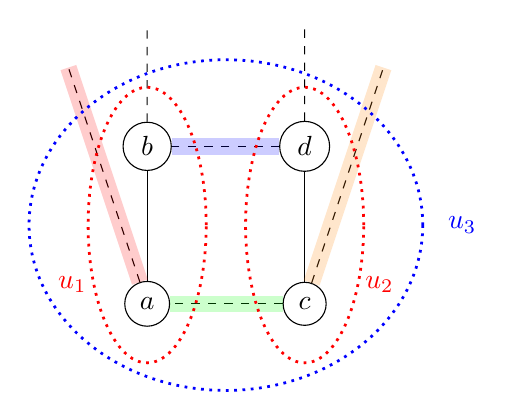
\begin{tikzpicture}
		\node [draw,circle] at (0,0) (a) {$a$};
		\node [draw,circle] at (0,2) (b) {$b$} edge (a);
		\node [draw,circle] at (2,0) (c) {$c$} edge [dashed] (a) edge [color=green,line width=6pt,opacity=0.2] (a) ;
		\node [draw,circle] at (2,2) (d) {$d$} edge (c) edge [dashed] (b) edge [line width=6pt,opacity=0.2,color=blue] (b);
		\draw [dashed] (a) -- +(-1,3)  (b) -- +(0,1.5) (d) -- +(0,1.5) (c) --  +(1,3);
		\draw [color=red,line width=6pt,opacity=0.2] (a) -- +(-1,3);
		\draw [color=orange,line width=6pt,opacity=0.2] (c) --  +(1,3);
		\draw [dotted,line width=1pt, color=red] (0,1) ellipse (0.75 and 1.75)
			(2,1) ellipse (0.75 and 1.75);
		\draw[line width=1pt,dotted,color=blue]	(1,1) ellipse (2.5 and 2.1);
		\node [color=red]at (-0.95,0.25) () {$u_1$};
		\node [color=red] at (2.95,0.25) () {$u_2$};
		\node [color=blue] at (4,1) () {$u_3$};
		
	\end{tikzpicture}
	\quad \quad \quad
	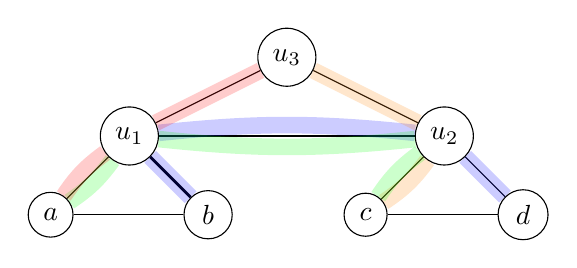
\begin{tikzpicture}
		\node [circle,draw] at (0,0) (a) {$a$};
		\node [circle,draw] at (2,0) (b) {$b$} edge (a);
		\node[circle,draw]  at (1,1) (u1) {$u_1$} edge (a) edge [color=green,opacity=0.2,line width=6pt,bend left=10] (a) edge [opacity=0.2,line width=6pt,color=red,bend right=10] (a) edge [line width=1pt](b) edge [color=blue,opacity=0.2,line width=6pt](b);
		\node[circle,draw]  at (4,0) (c) {$c$};
		\node [circle,draw] at (6,0) (d) {$d$} edge (c);
		\node [circle,draw] at (5,1) (u2) {$u_2$} edge (c) edge [color=orange,line width=6pt,opacity=0.2,bend left=10] (c) edge [color=green,opacity=0.2,line width=6pt,bend right=10] (c) edge (d) edge [color=blue,opacity=0.2,line width=6pt] (d) edge (u1) edge [color=blue,opacity=0.2,line width=6pt,bend right=6] (u1) edge [color=green,opacity=0.2,line width=6pt,bend left=6] (u1);
		\node[circle,draw]  at (3,2) (u3) {$u_3$} edge (u1) edge [color=red,opacity=0.2,line width=6pt] (u1) edge (u2) edge [color=orange,line width=6pt,opacity=0.2] (u2) ;
	\end{tikzpicture}
	\caption{\small An example of part of a hierarchy with three "triangles". The graph on the left shows part of a feasible LP solution where dashed (and sometimes colored) edges have fraction $1/2$ and solid edges have fraction 1. The dotted ellipses on the left show the min-cuts $u_1,u_2,u_3$ in the graph. (Each vertex is also a min-cut). On the right is a representation of the corresponding hierarchy. Triangle $u_1$ corresponds to the cut $\{a,b\}$, $u_2$ corresponds to $\{c,d\}$ and $u_3$ corresponds to $\{a,b,c,d\}$. Note that, for example, the edge $\{a,c\}$, represented in green,  is in $\delta(u_1)$,  $\delta(u_3)$, and inside $u_3$. In this example, $\p (\{a,b\}) = u_1$ and  $\p (\{a,c\}) = u_2$. Triangle $u_1$ is happy if $(\delta(a)\smallsetminus \{a,b\})_T = (\delta(b)\smallsetminus \{a,b\})_T = 1$.  }
	\label{fig:hierarchywithtriangle}
\end{figure}


 


 Our main remaining task is to explain how to use the hierarchy $\cH$ to choose a slack vector $s$ that has {\em negative} expected value, specifically, has $\E{s_e} = -\Omega(\decrease x_e)$ for each edge, while ensuring that all $O$-Join constraints coming from $\cH$ are satisfied. %Therefore by the above arguments, combining $s_e$ and $s_e^*$ ensures that \textit{all} constraints coming from $\cN_{\eta}$ are satisfied, and moreover since $-\E{s_e} \gg \E{s_e^*}$ we have $\E{s_e + s^*_e}$ sufficiently negative for $\eta$ small enough.

 %We now briefly review how \cite{KKO21} used the hierarchy and the sampled tree to construct a good slack vector $s$. 
 As mentioned in \cref{sec:overview}, the approach taken is to set $s_e$ to be negative (i.e. {\em reduce} it) when certain special cuts $e$ is on are even in the tree and therefore induce no $O$-join constraint. Roughly speaking, it works as follows: For each LP edge $f$, consider the lowest cut $S$ in the hierarchy that contains both endpoints of $f$. We call this cut $\p(f)$ (for "parent of $f$").
  Let $\bbe = \{u,v\}$ (where $u$ and $v$ are children of $S$ in $\cH$; recall $u,v$ are subsets of vertices) be the set of all edges $f = \{u', v'\}$ such that $u' \in u$ and $v' \in v$. 
  
 Cuts in $\cH$ are separated into three types. If $S \in \cH$ has at least three children and it is not an outer polygon cut, call it a \textit{degree cut}. If it has exactly two children, call it a \textit{triangle cut}. The remaining cuts, as defined above, are outer polygon cuts.

 If $\p(f)$ is a degree cut, then  set $s_f :=  - 0.57\decrease x_f$ for all $f \in \bbe$ whenever the event that $\delta(u)_T$ and $\delta(v)_T$ are both even in the tree occurs. Call $f$ ``good" if this event occurs with constant probability. Furthermore, it is shown that every cut $u$ with $\p(u)$ a degree cut contains a $\Omega(1)$ fraction of good edges.
% It is shown that for every cut $u$ (with $\p(u)$ a degree cut), the probability of this good event is $\Omega(1)$ for a subset of ``good" edges $G \subseteq \delta(S)$ where $x(G) \ge \Omega(1)$. 
 
 On the other hand, when $\p(f)$ is an outer polygon cut or a "triangle" cut (see \cref{fig:hierarchywithtriangle}), set $s_f = -  \decrease x_f$ for all $f \in \bbe$ whenever $p(f)$ is happy (as defined above).   Thus, when a polygon  is happy, {\em all} edges $e$ whose parent is that cut have their slack $s_e$ reduced simultaneously. %(and at an expected cost of $O(\eta\decrease x_e)$ per edge, all near min cuts internal to the polygon are simultaneously satisfied). 
 Moreover, the event that $p(f)$ is happy for a polygon cut (or triangle cut) occurs with constant probability.
    
However, regardless of the type of cut $p(f)$ is,   setting $s_f$ to a negative value can be problematic for the feasibility of other cuts lower down in the hierarchy that contain $f$. Therefore, when a cut $S'$ lower down in the hierarchy such that $f \in \delta(S')$ is  odd in the tree, the slack of {\em other} edges  in $\delta(S')$ are increased to compensate for the reduction in $s_f$, (i.e., to maintain feasibility of $y$ for the cut $S'$). 
 
 The challenge is to do all of this in a way that still guarantees that  overall $\E{s_e} < - \eps \decrease x_e$, while simultaneously ensuring that for any cut $S \in \cH$ if $\delta(S)_T$ is odd, $\sum_{e \in \delta(S)} s_e \ge 0$. Showing this is involved and requires careful probabilistic arguments that rely on the fact that the tree is sampled from a max-entropy distribution. We refer the reader to \cite{KKO21} for the details.
 
 %$S \in \cN_{\eta,\le 1}$, if $\delta(S)_T$ is odd, $\sum_{e \in \delta(S)} (s_e + s_e^*) \ge 0$. 
 
 
 \subsection{Proof of \cref{thm:main} using \cref{thm:maintechnical}}\label{subsec:proofofmain}

\maintechnical*
%Here we show how our main theorem follows easily from \cref{thm:maintechnical}:
\begin{proof}[Proof of \cref{thm:main}]
Let $x^0$ be an extreme point solution of LP \eqref{eq:tsplp}, with support $E_0$ and let $x$ be $x^0$ restricted to $E$. By \cref{fact:sptreepolytope} $x$ is in the spanning tree polytope. 
Let $\mu=\mu_{\lambda^*}$ be the max entropy distribution with marginals $x$, and let $s,s^*$ be as defined in \cref{thm:maintechnical}.
We will define $y:E_0\to\R_{\geq 0}$ such that:
$$y_e=\begin{cases}
x_e/2+s_e+s^*_e & \text{if } e\in E\\
\infty & \text{if } e=e_0
\end{cases}
$$	
We will show that $y$ is a feasible solution
to \eqref{eq:tjoinlp}.
First, observe that for any $S$ where $e_0\in\delta(S)$, we have $y(\delta(S))\geq 1$. Otherwise, we assume $u_0,v_0\notin S$.
If $S$ is an $\eta$-near min cut and $\delta(S)_T$ is odd, then by property (ii) of \cref{thm:maintechnical}, we have
$$ y(\delta(S)) = \frac{x(\delta(S))}{2}+ s(\delta(S))+s^*(\delta(S))\geq 1.$$
On the other hand, if $S$ is not an $\eta$-near min cut, then
$$y(\delta(S)) \geq (\frac{1}{2}-\decrease)x(\delta(S)) \ge (\frac{1}{2}-\decrease) \cdot (2+\eta) = 1+\frac{\eta}{2}-2\decrease -\decrease \eta$$
where in the first inequality we used property (i) of \cref{thm:maintechnical} which gives $s_e\geq -x_e \decrease$ with probability 1 along with the fact that $s^*$ is non-negative.
Therefore, choosing $\beta = \frac{\eta}{4+2\eta}$ ensures that $y$ is a feasible $O$-join solution.

Finally, using $c(e_0)=0$ and part (iii) of \cref{thm:maintechnical},
\begin{align*}
\E{c(y)}&= c(x)/2 + \E{c(s)} +\E{c(s^*)}\\
&\leq c(x)/2 - \eps_P \decrease \cdot \frac{1}{3}c(x) +125\eta \cdot \decrease  \cdot c(x)\\
&\leq (1/2-\frac{1}{6}\eps_P\decrease) \cdot c(x)
\end{align*}
choosing $\eta$ such that 
\begin{equation}\label{eq:whatiseta}
 	125\eta= \frac{1}{6}\eps_P
 \end{equation}

Now, we are ready to bound the approximation factor of our algorithm.
First, since $x^0$ is an  extreme point solution of \eqref{eq:tsplp}, $\min_{e\in E_0} x^0_e\geq \frac{1}{n!}$. So, by \cref{thm:maxentropycomp}, in polynomial time\footnote{Since the claim that the integrality gap is bounded below $3/2$ does not depend on the running time, it may appear that this step is unnecessary. However, we need to discuss the running time here because we are giving a stronger result that the max entropy algorithm returns a solution of expected cost at most $(3/2-\eps)c(x)$ in polynomial time.} we can find $\lambda:E\to\R_{\geq 0}$ such that for any $e\in E$, $\PP{\mu_\lambda}{e}\leq x_e(1+\delta)$ for some $\delta$ that we fix later. It follows that
$$ \sum_{e\in E} |\PP{\mu}{e} - \PP{\mu_{\lambda}}{e}| \leq n\delta.$$
By stability of maximum entropy distributions (see  \cite[Thm 4]{SV19} and references therein), we have that $\norm{\mu-\mu_\lambda}_1\leq O(n^4\delta)=:q$. Therefore, {for some $\delta \ll n^{-4}$ we get} $\norm{\mu-\mu_{\lambda}}_1=q\leq \frac{\eps_P\eta}{100}$. That means that 
$$ \EE{T\sim\mu_{\lambda}}{\text{min cost matching}} \leq \EE{T\sim\mu}{c(y)}+  q (c(x)/2) \leq \left(\frac12-\frac{1}{6}\eps_P\decrease 
 + \frac{\eps_P \eta }{100}\right)c(x), $$
where we used that for any spanning tree the cost of the minimum cost matching on odd degree vertices is at most $c(x)/2$.
Finally, since $\EE{T\sim\mu_\lambda}{c(T)}\leq c(x)(1+\delta)$, $\eps_P=3.12\cdot 10^{-16}$, and $\eta=4.16 \cdot 10^{-19}$ (from \eqref{eq:whatiseta}) and $\decrease = \eta/(4+2\eta)$, we get a $3/2-10^{-36}$ approximation algorithm (compared to $c(x)$).
\end{proof}



